\documentclass[tikz,border=8pt]{standalone}
\usepackage{amsmath}
\usepackage{pgfplots}
\usepackage{xcolor}
\pgfplotsset{compat=1.18}

\definecolor{lineblue}{HTML}{2F6DB2}
\definecolor{linegray}{HTML}{555555}

\begin{document}
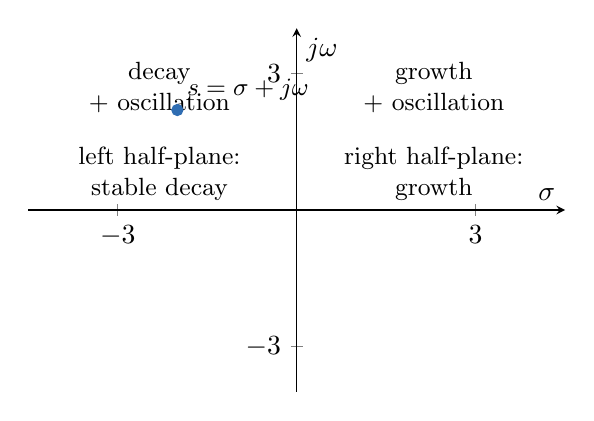
\begin{tikzpicture}
  \begin{axis}[
    width=8.4cm,
    height=6.2cm,
    xmin=-4.5, xmax=4.5,
    ymin=-4.0, ymax=4.0,
    axis lines=middle,
    xlabel={$\sigma$},
    ylabel={$j\omega$},
    xtick={-3,0,3},
    ytick={-3,0,3},
    clip=false
  ]
    \node[font=\small, align=center] at (axis cs:-2.3,2.7) {decay\\+ oscillation};
    \node[font=\small, align=center] at (axis cs:2.3,2.7) {growth\\+ oscillation};
    \node[font=\small, align=center] at (axis cs:-2.3,0.8) {left half-plane:\\stable decay};
    \node[font=\small, align=center] at (axis cs:2.3,0.8) {right half-plane:\\growth};
    \addplot[only marks, mark=*, mark size=2pt, color=lineblue] coordinates {(-2,2.2)};
    \node[font=\small, anchor=south west] at (axis cs:-2,2.2) {$s=\sigma+j\omega$};
  \end{axis}
\end{tikzpicture}
\end{document}
